
\section{Apache Hive}

Hive is an open-source data warehouse system built on top of Hadoop. It supports queries in a  SQL-like declarative query language, which is compiled into a directed acyclic graph of MapReduce jobs to be executed on Hadoop. Like traditional databases, Hive stores data in tables consisting of rows, where each row consists of a specified number of columns. The query language, HiveQL is a subset of SQL that includes certain extensions, including multitable inserts, but lacks support for transactions, materialized views and has limited subquery support. 

Figure \ref{fig:hivearch} shows an overview of the architecture of Hive. A number of external interfaces are available including command line, web UI, Thrift, JDBC, and ODBC interfaces. The metastore is essentially analogous to a system catalog in an RDBMS and contains a database (often MySQL or Derby) with a namespace for tables, table metadata, and partition information. Table data is stored in an HDFS directory, while a partition of a table is stored in a subdirectory within that directory. Buckets can cluster data by column and are stored in a file within the leaf level directory of a table or partition. Hive allows data to be included in a table or partition without having to transform it into a standard format, saving time and space for large data sets. This is achieved with support for custom SerDe (serialization/deserialization) java interface implementations with corresponding object inspectors. 

\begin{figure}[t]
	\centering
	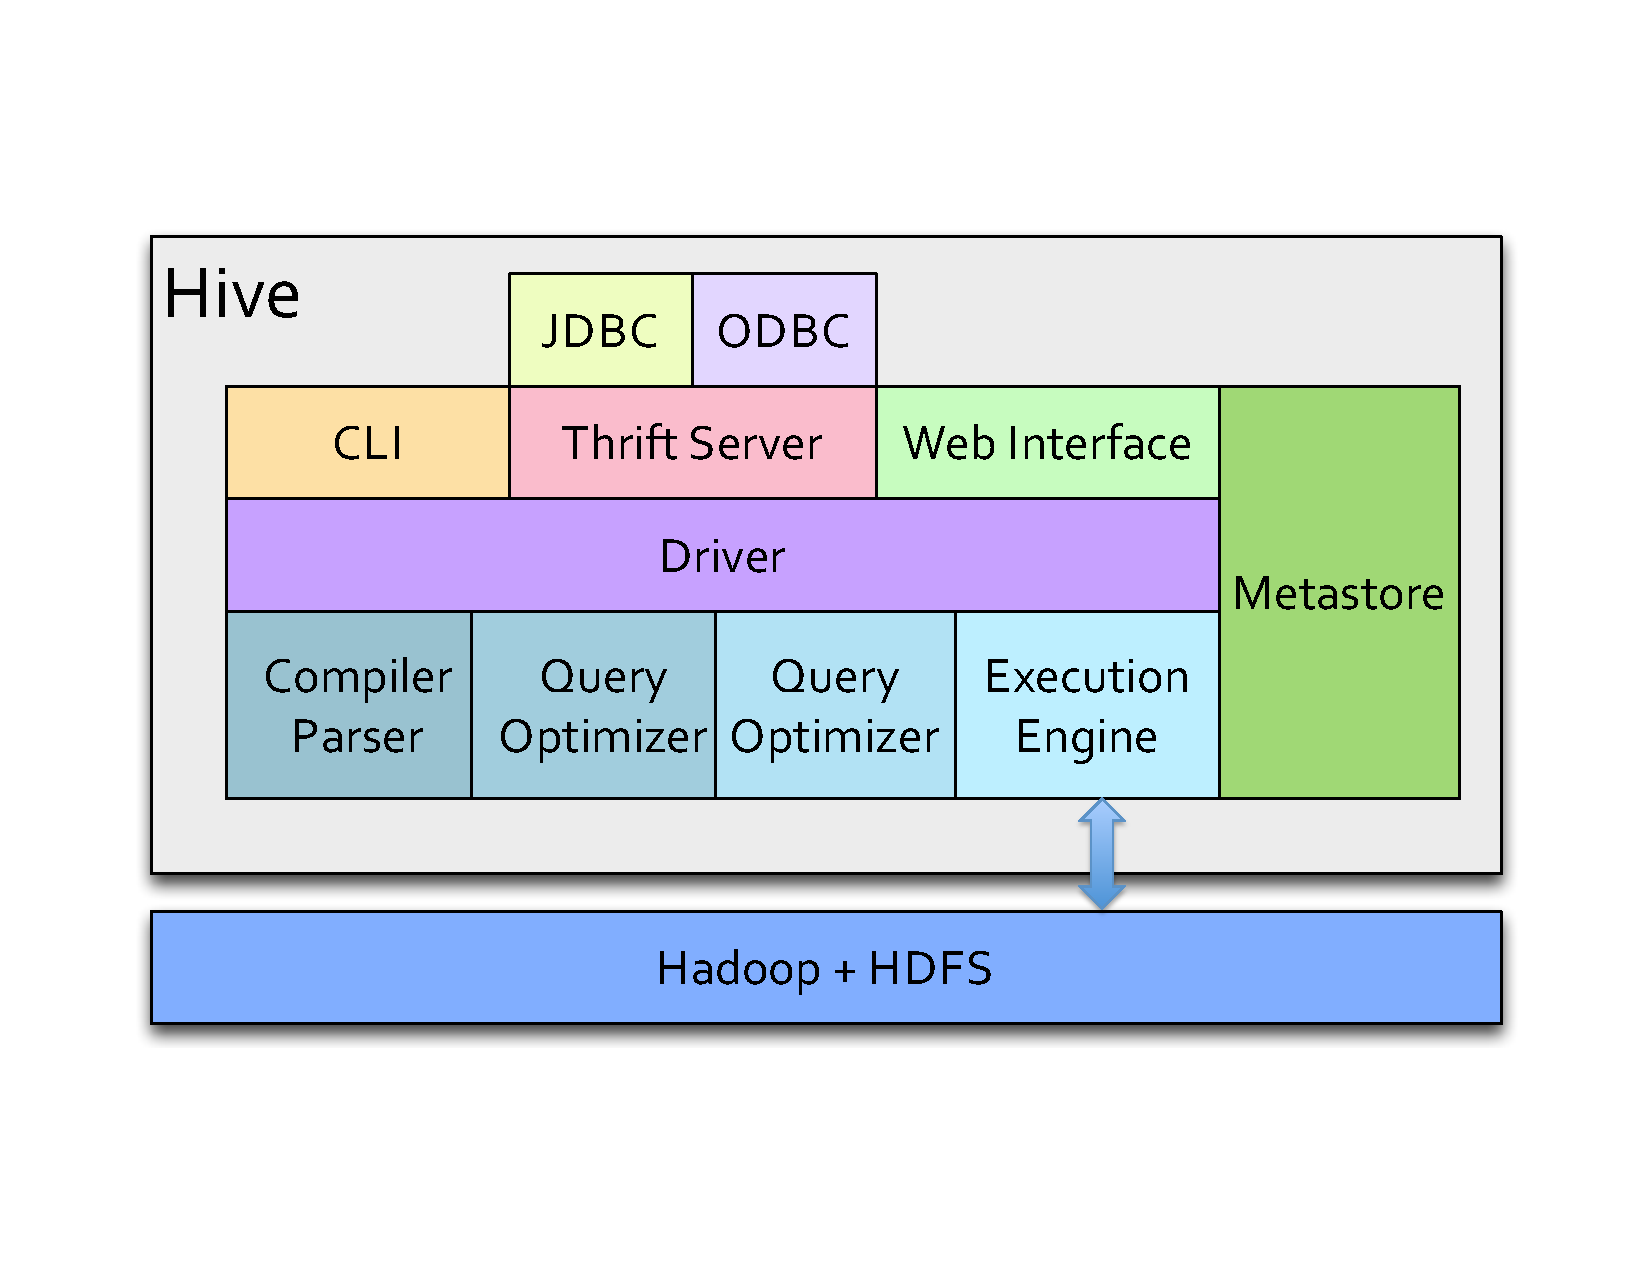
\includegraphics[width=\linewidth]{files/architecture-hive.pdf}
	\caption{Hive Architecture}
	\label{fig:hivearch}
\end{figure}


The Hive driver controls the processing of queries, coordinating their compilation, optimization, and execution. On receiving a HiveQL statement, the driver invokes the query compiler, which generates a directed acyclic graph (DAG) of map-reduce jobs for inserts and queries, metadata operations for DDL statements, or HDFS operations for loading data into tables. The Hive execution engine then executes the tasks generated by the compiler and interacts directly with Hadoop.

The generation of a query plan DAG shares many steps with a traditional database. A parser first turns a query into an abstract syntax tree (AST). The semantic analyzer turns the AST into an internal query representation and does type-checking and verifies column names. The logical plan generator then creates a logical plan as a tree of logical operators from the internal query representation. The optimizer rewrites the logical plan to add predicate pushdowns, early column pruning, repartition operators to mark boundaries between map and reduce phases, and to combine multiple joins on the same join key. The physical plan generator transforms the logical plan into a physical plan DAG of MapReduce jobs.
